%% This is an example first chapter.  You should put chapter/appendix that you
%% write into a separate file, and add a line \include{yourfilename} to
%% main.tex, where `yourfilename.tex' is the name of the chapter/appendix file.
%% You can process specific files by typing their names in at the 
%% \files=
%% prompt when you run the file main.tex through LaTeX.
\chapter{Design Options}
\label{ch:design}

GPU architecture is significantly different than that of a CPU, and thus a high performance PIC code on a GPU is going to look a lot different from its CPU equivalent. Memory access patterns, cache behavior, thread communication, and thread workload all have significant impacts on the performance of GPU codes. This means that porting an existing PIC code to the GPU is by no means straightforward, the data structures and algorithms will likely be different from the original serial code. 

Performance is just one facet of the code design, maintaining separate CPU and GPU versions of the same code presents additional problems. Programmers tend to be lazy in that the fewer lines of code that they have to write, the better. If a new feature is desired, then two different implementations of that feature must be written and debugged. From the lazy programmers perspective this is to be avoided as much as possible. Therefore, it is very important that the GPU version of the code utilize as much of the CPU code as possible. This means that interoperability between the CPU and GPU code must be both efficient and fast. 

Performance and maintenance are the two key issues that were considered when designing sceptic3Dgpu. Some of these issues have been investigated previously, although the amount of research in this area is still very small. To make matters worse, the specific techniques used are rapidly evolving with every new generation of graphics card. It is unlikely that the pace of GPU hardware evolution will slow in the near future. Spending large amounts of time optimizing algorithms for the current generation of hardware is inadvisable, and therefore the design of the code should focus on utilizing techniques that emphasize the underlying principles of GPU design or utilize library functions that will be optimized for each generation of hardware. 

The goal of this chapter is to outline various design options for implementing the various steps of the PIC algorithm on the GPU and explore the pros and cons of each option. Solutions used by other researchers will be outlined and evaluated based on their applicability to sceptic3D and their applicability to PIC codes in general. To accelerate these evaluations a simple 3D sandbox PIC code was implemented on the GPU in addition to several other basic comparison codes. 

%%%%%%%%%%%
%This means that separate CPU and GPU versions of the code must be maintained depending on the features desired for each architecture. Maintaining two separate versions of a code and as such it is important that the focus of GPU PIC code development be focused on steps of the PIC algorithm that are the most computationally intensive. Steps should be taken during the development to 


%For a serial or even MPI PIC implementations there is enough memory that each thread can have a separate copy of the grid and only need to talk to one another after chugging through a massive list of particles. In these cases the communications costs are negligible compared to the computations performed by each thread. On the GPU the situation is a lot different. Instead of a few threads doing lots of work you have a lot of threads doing little work. 
%%%%%%%%%%%
%%%%%%%%%%%%%%%%%%%%%%%%%%%%%%%%%%%%
	\section{GPUPIC Sandbox and the big questions}
%%%%%%%%%%%%%%%%%%%%%%%%%%%%%%%%%%%%
The first step in the development of sceptic3Dgpu was to create a very simple, generalized pic code that performed the major steps of the PIC algorithm and implement it in CUDA. This simple code, we'll call it GPUPIC\_testbed is designed without making any assumptions about the physics of the system. GPUPIC\_testbed operates in Cartesian coordinates with periodic boundary conditions. We do not really care too much about the field solve since in the serial version it takes a very small amount of time compared to the particle advance and charge assign steps. By recognizing the low priority of the field solve we really only need to characterize the performance of the following 5 steps:


\begin{enumerate}\itemsep0pt \parskip0pt \parsep0pt
\item Read the particle data
\item Read the Potential data for that particle
\item Move the particle
\item Write the new particle data back to the particle list
\item Interpolate Charge to Mesh
\item Goto 1
\end{enumerate}



The first implementation of this code was very naive. The only real difference from a serial version was the density array update, which used atomic updates on global memory in order to prevent memory collisions between multiple threads. Other than that the code boiled down to unrolling the loop over all of the particles into one particle per thread. The runtime breakdown of this code for a $32^3$ grid and 4.2 million particles is shown in table \ref{tab:GPUPIC_basetime}.


\begin{figure}
\begin{center}
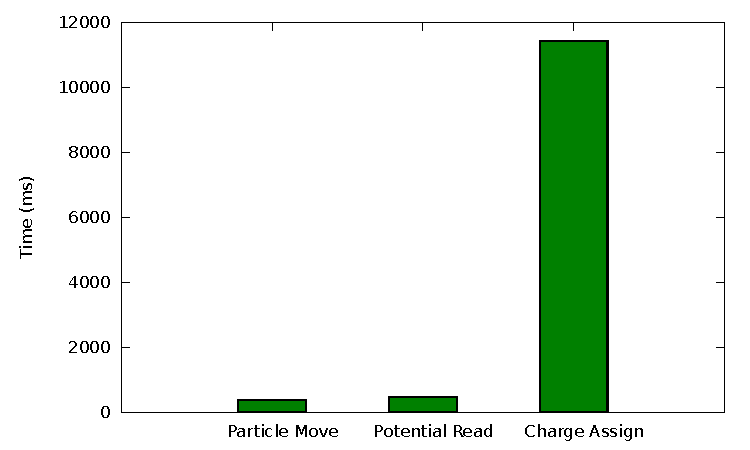
\includegraphics[width=5in]{design/sandbox_run_histo.pdf}
\end{center}
\caption{Total Execution times for 100 iterations of the key steps of the move kernel at three different optimizations.}
\label{fig:GPUPIC_basetime} 
\end{figure}



As you can see, the particle move and the potential read are very similar, but the charge assign is very slow. Determining how we can better adapt the charge assign to the GPU is our first major challenge. Several ways of dealling with the issue of the charge assign will be discussed in the following section. Some of the other issues that will be discussed in this chapter are:

\begin{itemize}\itemsep0pt \parskip0pt \parsep0pt
\item Particle Data Structure: Is it better to use an Array of structures, like the fortran code, or a Structure of Arrays?
\item How do we handle divergent processes in the advancing routine, such as losses, reinjections, and collisions?
\item At what point does the field solve become a dominant cost?
\item Are there any new issues that arise from solutions to the other issues?
\end{itemize}

%%%%%%%%%%%%%%%%%%%%%%%%%%%%%%%%%%%%
	\section{Charge Assign}
%%%%%%%%%%%%%%%%%%%%%%%%%%%%%%%%%%%%

There are two different ways to approach the charge assign, one in which information is ``pulled" from the particles by the vertices, and one in which data is ``pushed" by the particles to the vertices. Let G represent a grid of domain D of dimension d comprised of all vertices $v_s  \in \mathrm{D}$. We can define some distribution function $f(v_s)$ at each of the vertices which is the sum of some function $\mathrm{K}(v_s,p_i)$, where $p_i$ is the position of particle $i$. Given these definitions the algorithms for the particle pull and particle push method are algorithms \ref{alg:particle_pull} and \ref{alg:particle_push} respectively. 

\begin{algorithm}
	\begin{algorithmic}
		\STATE // Loop over the verticies first
		\FORALL{$\mathrm{vertex} \: v_s \in G$}
			\STATE find $\mathcal{P}(v_s)$
			\STATE $\mathrm{f}(v_s) \leftarrow 0$
			\FORALL{$p_i \in \mathcal{P}(v_s)$}
			\STATE $\mathrm{f}(v_s) \leftarrow \mathrm(f)(v_s) + \mathrm{K}(v_s,p_i)$
			\ENDFOR
		\ENDFOR
	\end{algorithmic}
	\caption{Particle Pull Method of charge deposition. From Stantchev et al. \cite{Stantchev2008}}
	\label{alg:particle_pull}
\end{algorithm}

\begin{algorithm}
	\begin{algorithmic}
		\STATE // Loop over the verticies first
		\FORALL{$\mathrm{vertex} \: v_s \in G$}
			\STATE $\mathrm{f}(v_s) \leftarrow 0$
		\ENDFOR
		\FORALL{$\mathrm{particle} \: p_i \in \mathrm{D}$}
			\STATE find $\mathcal{V}(p_i)$
			\FORALL{$v_s \in \mathcal{V}(p_i)$}
				\STATE $\mathrm{f}(v_s) \leftarrow \mathrm(f)(v_s) + \mathrm{K}(v_s,p_i)$
			\ENDFOR
		\ENDFOR
	\end{algorithmic}
	\caption{Particle Push Method of charge deposition. From Stantchev et al. \cite{Stantchev2008}}
	\label{alg:particle_push}
\end{algorithm}

As pointed out by \cite{Stantchev2008} each method has its advantages and disadvantages. For an algorithm consisting of N particles and k grid vertices the advantages and disadvantages are as follows:

The particle pull method
\begin{itemize}
\item requires $\mathcal{O}(2^dN + k)$ read write operations
\item $\mathcal{P}(v_s)$ is expensive to retrieve dynamically unless particles are organized
\end{itemize}

The particle push method
\begin{itemize}
\item requires $\mathcal{O}((2^d+1)N)$ read/write operations
\item $\mathcal{V}(p_i)$ is easily computed dynamically from the particles coordinates
\end{itemize}

The charge assign that we implemented in the sandbox PIC code is a particle push to an array in global memory. In that implementation we used atomic opperations to prevent memory collisions. Looking back at table \ref{tab:GPUPIC_basetime} we notice that the charge assign step constitutes about 93\% of the total runtime.  Unfortunately this poor performance is a result of serialization caused by the atomic updates. Additionaly, since the grid is far too large to fit in shared memory these updates must be performed on global memory, which has much higher latency and lower bandwidth. When a thread attempts to update a value in memory and finds that it is locked it must then repeat the process until it succeeds. Every failed update represents an additional slow global memory access that is essentially wasted. 

\begin{figure}
\begin{center}
% Turing Machine
% Author: Sebastian Sardina
%\documentclass[a4paper,10pt]{article}
%\documentclass{standalone}

%\begin{document}
\begin{tikzpicture}
\tikzstyle{every path}=[very thick]

\edef\sizetape{1.0cm}
\tikzstyle{tmtape}=[draw,minimum size=\sizetape]
\tikzstyle{tmtape1}=[draw,fill=Gray,minimum size=\sizetape]
\tikzstyle{tmhead}=[arrow box,draw,minimum size=.5cm,arrow box
arrows={east:.25cm, west:0.25cm}]

\tikzstyle directed=[postaction={decorate,decoration={markings,
    mark=at position .65 with {\arrow[arrowstyle]{stealth}}}}]

\tikzstyle arrowstyle=[scale=1]

\tikzstyle{cfill1}=[fill=Purple]
\tikzstyle{cfill2}=[fill=SkyBlue]
\tikzstyle{cfill3}=[fill=Maroon]
\tikzstyle{cfill4}=[fill=Emerald]

%% Draw TM tape
\begin{scope}[start chain=1 going right,node distance=-0.15mm]
    \node [on chain=1,tmtape,draw=none] {$\ldots$};
    \node [on chain=1,tmtape1] (input) {};
    \node [on chain=1,tmtape1,cfill1] (i0) {i};
    \node [on chain=1,tmtape1,cfill1] (i1) {i+1};
    \node [on chain=1,tmtape1,cfill2] (i2) {i+2};
    \node [on chain=1,tmtape1,cfill3] (i3) {i+3};
    \node [on chain=1,tmtape1,cfill4] (i4) {i+4};
    \node [on chain=1,tmtape1,cfill4] (i5) {i+5};
    \node [on chain=1,tmtape1] {};
    \node [on chain=1,tmtape,draw=none] {$\ldots$};
    \node [on chain=1] {\textbf{Particle stream}};

\end{scope}
\begin{scope}
[shift={(1.25cm,-3cm)},start chain=1 going right,node distance=-0.15mm]
    \node [on chain=1,tmtape,draw=none] {$\ldots$};
    \node [on chain=1,tmtape] (input) {};
    \node [on chain=1,tmtape,cfill1] (j1) {j};
	 \node [on chain=1,tmtape,cfill2] (j2) {j+1};
	 \node [on chain=1,tmtape,cfill3] (j3) {j+2};
	 \node [on chain=1,tmtape,cfill4] (j4) {j+3};
    \node [on chain=1,tmtape] {};
    \node [on chain=1,tmtape,draw=none] {$\ldots$};
    \node [on chain=1] {\textbf{Density Array}};
	

		

	%\draw[directed,dashed,red] (i0) -- (j1);	
	%\draw[directed,dashed,red] (i1) -- (j1);	
	%\draw[directed,dashed] (i2) -- (j2);
	%\draw[directed,dashed] (i3) -- (j3);	
	%\draw[directed,dashed,red] (i4) -- (j4);
	%\draw[directed,dashed,red] (i5) -- (j4);	
	\path[dashed,red] (i0) edge [directed,out=-90, in=90] (j1);	
	\path[dashed,red] (i1) edge [directed,out=-90, in=90] (j1);	
	\path[dashed] (i2) edge [directed,out=-90, in=90] (j2);
	\path[dashed] (i3) edge [directed,out=-90, in=90] (j3);	
	\path[dashed,red] (i4) edge [directed,out=-90, in=90] (j4);
	\path[dashed,red] (i5) edge [directed,out=-90, in=90] (j4);	
	%\draw[color=red] (j4)	circle (0.7cm);
	%\draw[color=red] (j1)	circle (0.7cm);

	\path ++(j1)++(90:0.6cm) coordinate (c1);
	\path ++(j4)++(90:0.6cm) coordinate (c2);
	\path ++(j4)++(4cm,1.25cm) node [red] {\textbf{Memory Conflicts}};
	\path ++(j4)++(2cm,1.25cm) coordinate (c4);
	\path ++(j4)++(1.5cm,1.25cm) coordinate (c3);

	\draw[->,color=red] (c1) -- (c3) -- (c4);
	\draw[->,color=red] (c2) -- (c3) -- (c4);
\end{scope}


\end{tikzpicture}
%\end{document}


\end{center}
\caption{Atomic Memory collisions}
\label{fig:pic_flowchart_parallel}
\end{figure}

The technique applied for MPI codes is parallel reduction. Each thread deals with a subset of the particle list and tallies up the contributions of that list to some array in memory private to a single thread. Once every thread has recorded the contributions from their subset of the particle list a parallel reduction is performed in order to quickly sum up the contributions from all threads. The problem with directly applying this solution to the GPU is that when a thread reads in a particle the thread must be able to account for every possible location that the particle can contribute to. With a completely random particle list any given particle can contribute to any element of the grid. However, say a thread knows that every particle that it reads in will only contribute to one element of the grid. This thread now only has to keep track of a single value, since it knows that every particle it sees will only contribute to this value. When it comes time for all of the threads to contribute to the final result each thread provides the full answer for a single element. This is essentially the particle pull method described in algorithm \ref{alg:particle_pull} without the need to to retrieve $\mathcal{P}(v_s)$ dynamically. One of the main benefits to this method is that it significantly reduces the memory requirements of each thread but imposes the constraint that a thread is given only particles that exist within its domain. We will worry about this additional constraint later. 

\begin{figure}
\begin{center}
% Turing Machine
% Author: Sebastian Sardina
%\documentclass[a4paper,10pt]{article}
%\usepackage[usenames,dvipsnames]{xcolor}
%\usepackage{tikz}
%\usetikzlibrary{chains,fit,shapes}
%\begin{document}


\begin{tikzpicture}\noindent

\node [shift={(0cm,0cm)}]
	{
		\begin{tikzpicture}[remember picture]
\tikzstyle{every path}=[very thick]

\edef\sizetape{1.0cm}
\tikzstyle{tmtape}=[draw,minimum size=\sizetape]
\tikzstyle{tmtape1}=[draw,minimum size=\sizetape]
\tikzstyle{tmhead}=[arrow box,draw,minimum size=0.8cm,arrow box
arrows={east:.25cm}]

\tikzstyle{cfill1}=[fill=Purple]
\tikzstyle{cfill2}=[fill=SkyBlue]
\tikzstyle{cfill3}=[fill=Maroon]
\tikzstyle{cfill4}=[fill=Emerald]



%% Draw Density Array
\begin{scope}[start chain=1 going right,node distance=-0.15mm]
    \node [on chain=1,tmtape,draw=none] {$\ldots$};
    \node [on chain=1,tmtape,fill=Gray] (input) {};
    \node [on chain=1,tmtape,cfill1] (j1) {j};
	 \node [on chain=1,tmtape,cfill2] (j2) {j+1};
	 \node [on chain=1,tmtape,cfill3] (j3) {j+2};
	 \node [on chain=1,tmtape,cfill4] (j4) {j+3};
    \node [on chain=1,tmtape,fill=Gray] {};
    \node [on chain=1,tmtape,draw=none] {$\ldots$};
    \node [on chain=1] {\textbf{Density Array}};


\end{scope}

\begin{scope}[shift={(-1cm,-4cm)},start chain=1 going right,node distance=-0.15mm]

    \node [on chain=1,tmtape,draw=none] {$\ldots$};
    \node [on chain=1,tmtape1,cfill1] (input) {i};
    \node [on chain=1,tmtape1,cfill1] (i0) {i+1};
	 \node [on chain=1,tmtape,draw=none] {$\ldots$};
    \node [on chain=1,tmtape1,cfill2] (i1) {i+2};
    \node [on chain=1,tmtape1,cfill2] (i2) {i+3};
	 \node [on chain=1,tmtape,draw=none] {$\ldots$};
    \node [on chain=1,tmtape1,cfill3] (i3) {i+4};
    \node [on chain=1,tmtape1,cfill3] (i4) {i+5};
 	 \node [on chain=1,tmtape,draw=none] {$\ldots$};
    \node [on chain=1,tmtape1,cfill4] (i5) {i+6};
    \node [on chain=1,tmtape1,cfill4] {i+7};
    \node [on chain=1,tmtape,draw=none] {$\ldots$};
    \node [on chain=1] {\textbf{Particle stream}};
	
\end{scope}

\node [tmhead,yshift=0.45cm] at (input.north) (head1) {$T_1$};
\node [tmhead,yshift=0.45cm] at (i1.north) (head2) {$T_2$};
\node [tmhead,yshift=0.45cm] at (i3.north) (head3) {$T_3$};
\node [tmhead,yshift=0.45cm] at (i5.north) (head4) {$T_4$};
		

	\path[->] (head1) edge [out=90, in=-90] (j1);	
	\path[->] (head2) edge [out=90, in=-90] (j2);
	\path[->] (head3) edge [out=90, in=-90] (j3);	
	\path[->] (head4) edge [out=90, in=-90] (j4);	

	\end{tikzpicture}
	};
\end{tikzpicture}
%\end{document}


\end{center}
\caption{One thread per cell}
\label{fig:pic_flowchart_parallel}
\end{figure}

Now consider this, the MPI code works well for a few randomly ordered sets of many particles, or objects, manipulated by a small number of threads. The decomposition technique works for a small number of organized sets of a few objects manipulated a large number of threads. If we think of threads operating on small groups of particles as objects and we replace every instance of `objects' with `threads' in the previous two sentences we end up with an interesting situation. Apply the MPI technique to a few randomly ordered sets of many threads each operating on a small number of particles. Essentially if we want to run really large particle lists we can divide up the list amongst several nodes. Each node uses many threads to process a small ordered subset of this list and contribute to the full array. Once every node has completed its own tally the standard MPI technique is used to gather the tallies of all the nodes. This is an excellent example of multi-grained parallelism. The level consisting of multiple nodes is coarse parallelism while the node level is a finer level of parallelism.   

\begin{figure}
\begin{center}
% Turing Machine
% Author: Sebastian Sardina
%\documentclass[a4paper,10pt]{article}
%\usepackage[usenames,dvipsnames]{xcolor}
%\usepackage{tikz}
%\usetikzlibrary{chains,fit,shapes}
%\begin{document}

\noindent
\begin{tikzpicture}
		\tikzstyle{every path}=[very thick]

		\edef\sizetape{1.0cm}
		\tikzstyle{tmtape}=[draw,minimum size=\sizetape]
		\tikzstyle{tmtape1}=[draw,minimum size=0.4cm]
		\tikzstyle{tmhead}=[arrow box,draw,minimum size=0.4cm,arrow box
		arrows={east:.25cm}]

		\tikzstyle{cfill1}=[fill=Purple]
		\tikzstyle{cfill2}=[fill=SkyBlue]
		\tikzstyle{cfill3}=[fill=Maroon]
		\tikzstyle{cfill4}=[fill=Emerald]

\node [shift={(-1.0cm,-2cm)}]
	{
		\begin{tikzpicture}[remember picture]



					\begin{scope}[start chain=2 going below,start chain=1 going right,node distance=-0.15mm] at (current page.north west)
						 \node [on chain=2,yshift=0.5cm] {Particle Stream};
						 \node [on chain=1,tmtape1,draw=none,xshift=-5cm] {$\ldots$};
						 \node [on chain=1,tmtape1,cfill1] (input) {};
						 \node [on chain=1,tmtape1,cfill4] (i0) {};
						 \node [on chain=1,tmtape1,cfill3] (i3) {};
						 \node [on chain=1,tmtape1,cfill2] (i4) {};
						 \node [on chain=1,tmtape1,cfill1] (i5) {};
						 \node [on chain=1,tmtape1,cfill4] {};
						 \node [on chain=1,tmtape,draw=none] {$\ldots$};
						 \node [on chain=1,tmtape1,cfill3] (i6) {};
						 \node [on chain=1,tmtape1,cfill2] (i7) {};
						 \node [on chain=1,tmtape1,cfill1] (i8) {};
						 \node [on chain=1,tmtape1,cfill3] (i9) {};
						 \node [on chain=1,tmtape1,cfill4] (i11) {};
						 \node [on chain=1,tmtape,draw=none] {$\ldots$};
						 \node [on chain=1,tmtape1,cfill4] (i11) {};
						 \node [on chain=1,tmtape1,cfill3] (i12) {};
						 \node [on chain=1,tmtape1,cfill2] (i13) {};
						 \node [on chain=1,tmtape1,cfill4] (i16) {};
						 \node [on chain=1,tmtape1,cfill1] (i17) {};
						 \node [on chain=1,tmtape,draw=none] {$\ldots$};
						 
					\end{scope}

		\node [tmhead,yshift=-0.45cm] at (input.south) (head1) {$T_1$};
		\node [tmhead,yshift=-0.45cm] at (i6.south) (head2) {$T_2$};
		\node [tmhead,yshift=-0.45cm] at (i11.south) (head3) {$T_3$};

		
		\footnotesize
		\node [xshift=-3cm,yshift=-5cm] (a1)
			{\begin{tikzpicture}[remember picture]
			\begin{scope}[start chain=1 going right,start chain=3 going down,start chain=2 going right,node distance=-1.0mm]

				 \node [on chain=1,tmtape,cfill1] (j1) {j};
				 \node [on chain=1,tmtape,cfill2] (j2) {j+1};
				 \node [on chain=2,tmtape,cfill3,yshift=-.985cm] at (j1) (j3) {j+2};
				 \node [on chain=2,tmtape,cfill4] (j4) {j+3};
				 \node [on chain=3,yshift=-0.75cm,xshift=-0.5cm] at (j4) {Array 1};  

			\end{scope}
			\end{tikzpicture}
			};

		\node [shift={(3cm,0cm)}] at (a1) (a2)
			{\begin{tikzpicture}[remember picture]
			\begin{scope}[start chain=1 going right,start chain=3 going down,start chain=2 going right,node distance=-1.0mm]
   
				 \node [on chain=1,tmtape,cfill1] (j5) {j};
				 \node [on chain=1,tmtape,cfill2] (j6) {j+1};
				 \node [on chain=2,tmtape,cfill3,yshift=-.985cm] at (j5) (j7) {j+2};
				 \node [on chain=2,tmtape,cfill4] (j8) {j+3};
				 \node [on chain=3,yshift=-0.75cm,xshift=-0.5cm] at (j8) {Array 2};  

			\end{scope}
			\end{tikzpicture}
			};

		\node [shift={(3cm,0cm)}] at (a2)
			{\begin{tikzpicture}[remember picture]
			\begin{scope}[start chain=1 going right,start chain=2 going right,start chain=3 going down,node distance=-1.0mm]

				   
				 \node [on chain=1,tmtape,cfill1] (j9) {j};
				 \node [on chain=1,tmtape,cfill2] (j10) {j+1};
				 \node [on chain=2,tmtape,cfill3,yshift=-.985cm] at (j9) (j11) {j+2};
				 \node [on chain=2,tmtape,cfill4] (j12) {j+3};
				 \node [on chain=3,yshift=-0.75cm,xshift=-0.5cm] at (j12) {Array 3};  

			\end{scope}
			\end{tikzpicture}
			};





			\path[->] (head1) edge [bend right] (j1);	
			\path[->] (head2) edge [out=-90, in=180] (j7);
			\path[->] (head3) edge [out=-90, in=45] (j12);	

			\end{tikzpicture}
	};
\end{tikzpicture}
%\end{document}


\end{center}
\caption{MPI and One thread per cell}
\label{fig:pic_flowchart_parallel}
\end{figure}

We can take this methodology even further on the GPU by recognizing that we can parallelize the single element summations using reductions. Taking this to the limit of one thread per particle on the GPU we end up with each thread block, or several blocks, is responsible for a subset of the particle list. All of the particles in the block's list will contribute to the same element. The threads within each block read in their particles contribution to that element into shared memory. With all of the data in shared memory a very fast parallel reduction can be performed.

\begin{figure}
\begin{center}
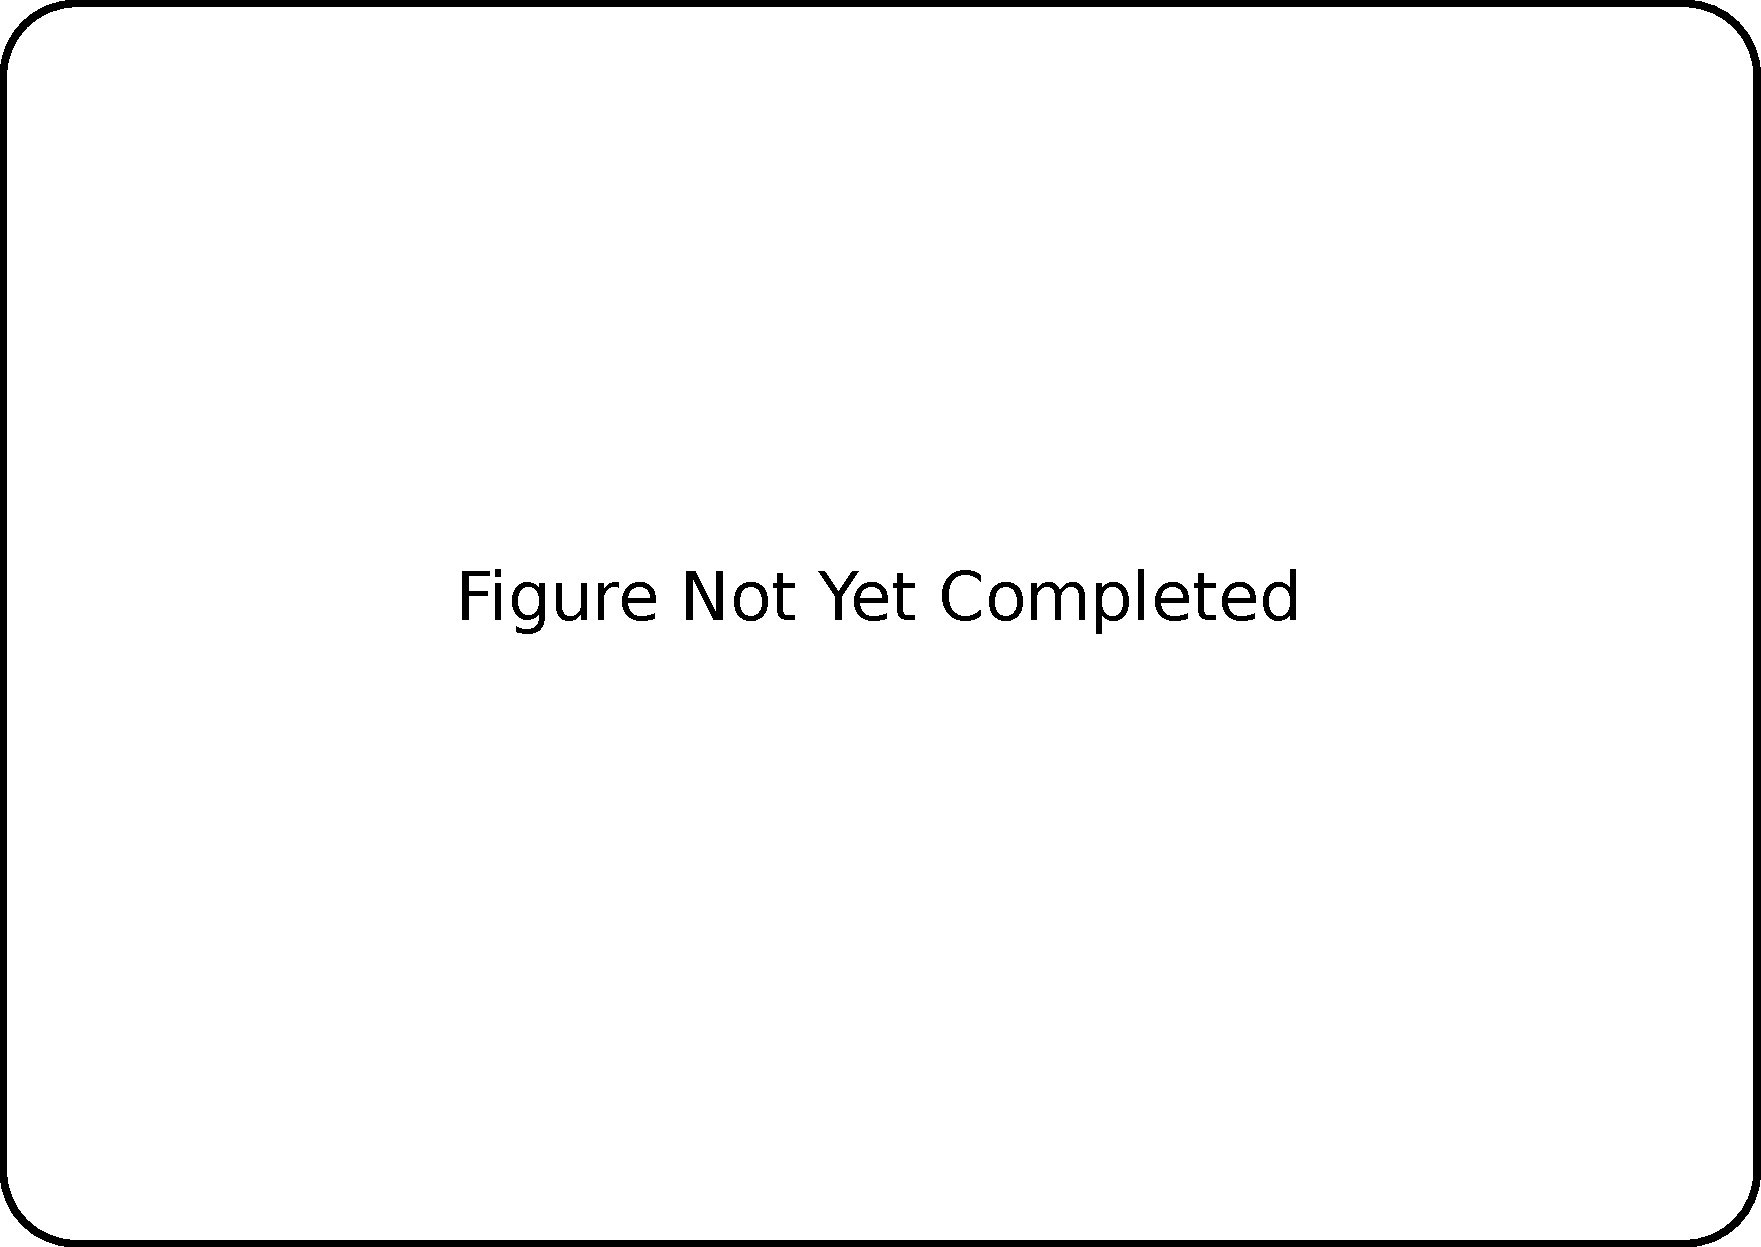
\includegraphics[width=5in]{introduction/not_finished.pdf}
\end{center}
\caption{Three levels of parallelism for the charge assign}
\label{fig:pic_flowchart_parallel}
\end{figure}

We implemented this technique in the sandbox PIC code and compared the runtime of the reduction particle-pull to the atomic particle-push. The results of this comparison can be seen in table \ref{tab:GPUPIC_comparison}.

\begin{figure}
\begin{center}
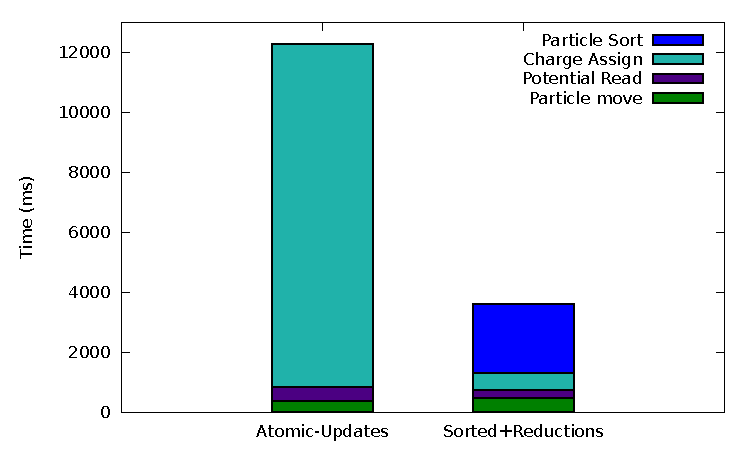
\includegraphics[width=5in]{design/atomic_vs_sorted.pdf}
\end{center}
\caption{Total Execution times for 100 iterations of the key steps of the move kernel at two different optimizations.}
\label{fig:GPUPIC_comparison}
\end{figure}




As you can see from the table, the charge assign is on the order of 20x faster using the reduction technique, although this speedup is somewhat offset by the sorting requirement. Sorting the particles also benefits reading the potential during the advancing step. This speedup is a result of increased cache hits due to all threads within the same thread block accessing the same addresses in the potential array. 

Although we have successfully reduced the cost of the charge assign we have introduced an additional cost of a sorting step\footnote{It should be noted that the sort used here is an older version of the radix sort, newer versions, such as the thrust implementation are much faster}. In the case of the sandbox code the sort step accounts for roughly 70\% of the runtime. Fortunately several other projects have figured out that there are ways reduce the sorting costs while maintaining some of the performance achieved by utilizing a sorted particle list. 

 
		\subsection{Other Codes}
There are several papers which point out that sorting by cell at every time step is not entirely necessary for the particle-pull method. It is possible to minimize the sorting requirement by expanding the sorting bins to include multiple cells, or rather, by dividing the simulation space into slabs composed of multiple cells. The advantage to this technique is sorting is only required between slabs, but not within the slabs.\cite{Abreu2011} 

This slab method, as described by Abreu et al, is used on a one thread per slab basis. One thread for each slab loops over all of the particles that belong to that slab, contributing to an array that is the same size as the slab. Once a thread completes its particle loop it writes the portion of the array that it is responsible for to the main array, using atomic operations for guard cells.\cite{Abreu2011} Similar approaches are used by Stantchev et al and Kong et al.\cite{Stantchev2008}\cite{Kong2011}

Unfortunately it is difficult to apply the reduction version of the particle push to the slab method. The reason this is difficult boils down to limited shared memory. Consider a slab with $nv_{slab}$ vertices. In order for the reduction to work we need to have $nv_{slab} * \mathrm{nthreads}$ floats to store the results of each thread. For a typical NVIDIA GPU with 49k shared memory per streaming multiprocessor and 128 threads per block, we are limited to a slab of about 96 vertices per slab. This amounts to 9 cells per slab for a 3D grid, or about 3 fewer steps for a radix sort.

The approaches used by Kong and Stantchev is a sort of hybridization of the push and pull algorithms. Here the grid is domain decomposed into sub-domains and each sub-domain assigned to a thread-block. Each thread-block has an array representing the distribution function for that sub-domain allocated in shared memory. Particles are ordered in the particle list according to what sub-domain they reside in. Within each sub-domain the charge assign is performed like a particle push. Threads loop through a subset of the particles, check which vertices that particle is updating, and update the distribution function at those vertices. 

In order to avoid memory collisions both Kong and Stantchev use a technique similar to atomic operations. The technique that they used is called thread-tagging and is no longer needed due to the addition of atomic operations for shared memory.\cite{Stantchev2008}\cite{Kong2011} This approach has several advantages over the reduction technique, the primary reasons being lower order sorting keys and slightly easier implementation. The disadvantage of this approach is that because it relies on atomic operations there is no guarantee that the results are deterministic since the order of the atomic operations is undefined. 







%%%%%%%%%%%%%%%%%%%%%%%%%%%%%%%%%%%%
	\section{Particle List Sort}
%%%%%%%%%%%%%%%%%%%%%%%%%%%%%%%%%%%%
		In the previous section we discussed what is required for an efficient charge assign on the GPU. In order to massively parallelize the charge assign and avoid memory collisions the particle data must be organized. Unfortunately this means introducing a new step in the PIC method, a sort step. Looking back at table \ref{tab:GPUPIC_comparison} we can see that this sort step is now the dominant cost by a large margin\footnote{Please note that these results are for the radix sort outlined in the NVIDIA GPU computing SDK version 3.1, developed by N. Satish et al.\cite{Satish2009}}. Operating with one step consuming 64\% of the total run time is unacceptable, we need to figure out a better way of keeping the particle data organized than this radix sort. Fortunately this problem has been explored in great detail by just about everyone else who has developed a GPU PIC implementation. 

Particle sorting for GPU PIC codes basically comes in four flavors:
\begin{itemize}
\item Partial sort using message passing. \cite{Kong2011}\cite{Decyk2011}
\item In-place particle Quicksort. \cite{Stantchev2008}
\item Linked list reordering \cite{Burau2010}
\item Full Radix Sort-by-key and reorder. \cite{Abreu2011}
\end{itemize}
Each of these methods have their own advantages and disadvantages. For the purposes of this code we are looking for a method that is fast for a broad range of applications and does not depend too greatly on the specifics of the problem.



	\subsection{Message Passing Sort}
	Going back a section to the charge assign we concluded that sorting by cell is unnecessary. Instead we are ordering the particles according to a group of cells called bins. For most cases the dimensions of the bin will be greater than the average distance that a particle will travel in a given time step. There are cases in which the particle path length will be smaller than the size of a cell, however this is much more likely if the domain in question is several cells wide. The benefit of considering this case is that only a small fraction of the particles will leave the domain during a given time step, and thus only a small number of particles need to be moved from one domain to the next. Most of the particles will remain in their respective domains and therefore do not need to be sorted. Instead of a full particle sort we want a method that will partially sort the particle list, only handling the particles that changed domains. 

	One partial sorting method is similar in principle to message passing. The particle list is divided up into sections according to domain. Whenever a particle leaves its current domain it is flagged. Flagged particles are then moved to different sections of the particle list through some kind of buffer. There are currently two approaches to this. The approach taken by Kong et al, illustrated in figure \ref{fig:kong_sort} is based on integrating the buffer into the particle list. The particle list is structured such that each sub-domain's section of the particle list is divided into two regions, a data region and a buffer region. Using this particle list structure as a foundation, the rest of the sorting algorithm proceeds as follows\cite{Kong2011}:

\begin{enumerate}
\singlespace
\item Sub-domains, referred to by Kong as clusters, that are adjacent horizontally are grouped into pairs called bi-clusters. This first step is odd cells on the left, even cells on the right. 
\item Particles that are moving from the left cluster to the right are copied from the left cluster into the buffer section of the right cluster. 
\item Step 2 is then repeated for particles moving from the right cluster to the left. 
\item Repeat steps 1 to 3 for bi-clusters for even cells on the left and odd cells on the right. 
\item Perform steps 1 to 4 for vertically oriented bi-clusters. 
\end{enumerate}


\begin{figure}
\begin{center}
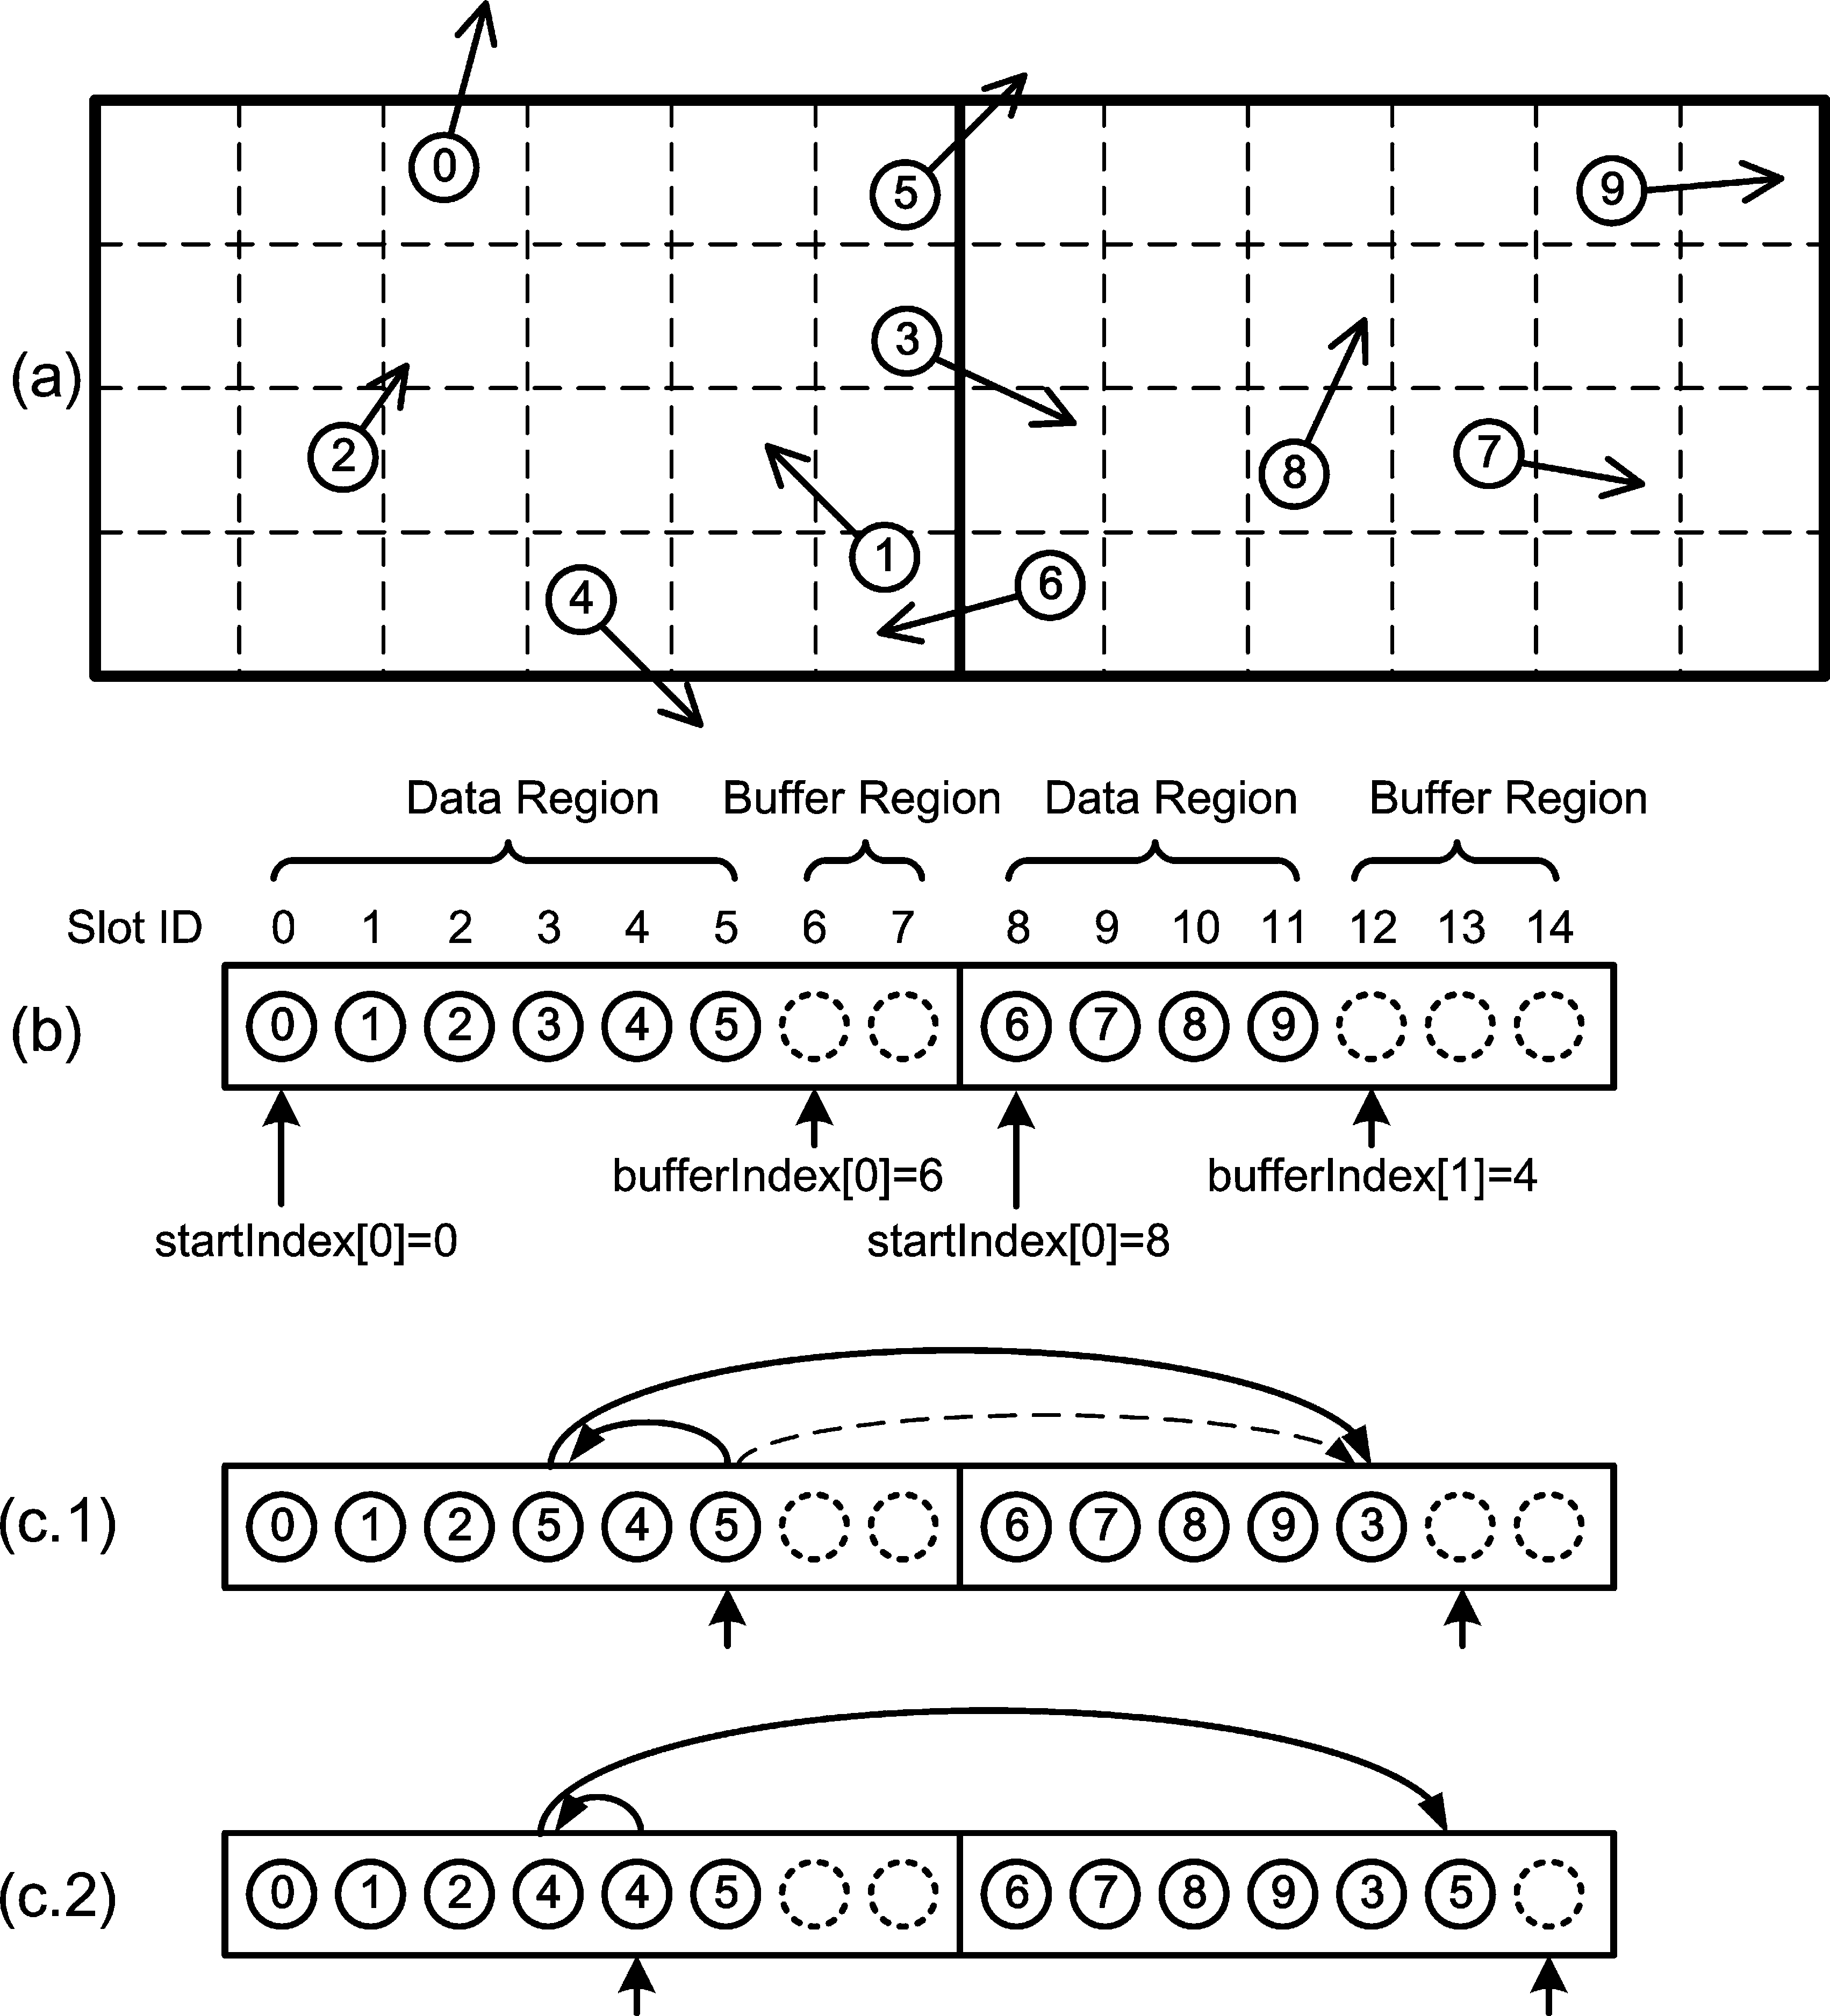
\includegraphics[width=5in]{design/kong_sort.png}
\end{center}
\caption{Kong particle sort. (a) Bi-cluster of cells. (b) Data structure of the bi-cluster particle array. (c.1) Particle 3 and 5 move to the right. Particle 3 is moved first to slot 12 which frees up slot 3. Slot 3, now empty, copies the last particle in the data region, which is particle 5. Particle 5 is also moving to the right so slot 3 copies it to slot 13 and replaces the contents of slot 3 with particle 4. Image taken from \cite{Kong2011}.}
\label{fig:kong_sort}
\end{figure}

	In cases where the number of particles in a cluster is greater than the number of slots in that cluster a global data reorder must be performed. This reorder is only performed when a particle to slot ratio exceeds a certain limit. When a cluster exceeds this threshold the code increases the buffer for this cluster by reducing the buffer of other clusters. This operation is carried out through a sequence of calls to $cudaMemcpy()$ where a section of data from end of a cluster is copied to the end of the buffer of the previous cluster. The start index of the adjusted cluster is then shifted by the amount of memory copied. \cite{Kong2011}

	This method works well if we assume that a particle will move at most one cluster in any direction in a single time step. If a particle moves more two clusters, then the sort must be performed twice, one for each step that the particle moves. In the worst case scenario, where a particle can move from one cluster to any other of n clusters, it may take up to $n$ sort steps to put every particle in its proper cluster. Another downside to this method is that it requires extra memory for the buffer. If the buffer is to small then global reorders will be performed more often. If the buffer section is too large then precious memory is wasted. 

	\subsection{In Place Particle-Quicksort}
	The second sort method, developed by George Stantchev et al, eliminates the need for a buffer array, and is applicable to cases in which particles can move any number of clusters. This sort, like the Kong sort, is an ``incomplete'' which reorders only those particles that have changed position. For this sort the particle list is divided up into ``bins" representing groups of cells to which particles in that bin belong. A separate array keeps track of the indicies, called ``bookmarks" of the first and last particle of each bin. The actually sorting is based on moving particles within their respective bins and manipulating the bookmarks such that in the end all particles are where they belong. The algorithm consists of two steps, a defragmentation step and a rebracketing step. 
	
	After the particle advance some of the particles will have moved to bins with a higher bin index, and some to bins with a lower. Since the particle list is laid out continiously in linear memory higher bins will be to the right, and lower bins to the left of the current bin. The purpose of the defragmentation step is to organize the particles within a bin into three subsets based on the direction that they are traveling, left, right, or staying. Let $P = [p_{i_1}.... p_{i_n}]$ represent a particle bin that maps to a group of cells $C$ with memory index $j$. The cell cluster that each particle resides in is denoted by $I(p)$. As shown in algorithm \ref{alg:defrag} the defragmentation is performed through two loops over all elements in $P$

\begin{algorithm}
	\begin{algorithmic}
		\STATE // Loop over particle bins
		\FORALL{particle bin $P_l$}
			\STATE $t_{min} \leftarrow$ lowest cell in the cluster associated with $P_l$
			\STATE $t_{max} \leftarrow$ highest cell in the cluster associated with $P_l$
			\STATE $\alpha \leftarrow$ lowest particle index of  $P_l$
			\STATE $\omega \leftarrow$ highest particle index of $P_l$
			\STATE // Forward Swapping pass 
			\FORALL{$p_i \in P_l in ascending order$}
				\IF{$I(p_i) < t_{min}$}
					\STATE swap$(p_i, p_{\alpha})$
					\STATE $\alpha \leftarrow \alpha + 1$
				\ENDIF			
			\ENDFOR
			\STATE Backward swapping pass
			\FORALL{$p_i \in P_l in descending order$}
				\IF{$I(p_i) > t_{max}$}
					\STATE swap$(p_i, p_{\omega})$
					\STATE $\omega \leftarrow \omega - 1$
				\ENDIF			
			\ENDFOR
			\STATE // Now $\alpha$ and $\omega$ are the new temporary bookmarks indicating the boundaries between migrating and non-migrating particles in bin $P_l$
		\ENDFOR
	\end{algorithmic}
	\caption{Particle defragmentation. From Stantchev et al. \cite{Stantchev2008}}
	\label{alg:defrag}
\end{algorithm}


 Once the defragmentation step is complete the subset of the particles that are migrating must be moved to their new homes and the particle bin bookmarks updated. This step, called particle rebracketing and shown in algorithm \ref{alg:rebracket}, is performed first for all odd $l$ and then for all even $l$. Each rebracketing step starts by taking two adjacent particle bins, $P_l$ and $P_{l+1}$. Particle $p_{\omega_l}$ in bin $P_{l}$ is swapped with particle $p_{\alpha_{l+1}}$ in bin $P_{l+1}$. After the swap $\alpha_{l+1}$ is decreased by 1 and $\omega_l$ is increased by 1. This is repeated until $I(p_{\omega_l}) = I(P_l)$. The final bookmark $l$, the final particle in bin $P_l$, is given by the original values of $\alpha_{l+1}$ and $\omega_l$, $l = \alpha_{l+1}^0 - l + \omega_l^0$. The process is then repeated for all even values of $l$.

\begin{algorithm}
	\begin{algorithmic}
		\STATE // Odd Particle bins
		\FORALL{particle bin $P_l$ where $l$ is odd}
			\STATE $\alpha \leftarrow \alpha_{l+1}^0$
			\STATE $\omega \leftarrow \omega_l^0$
			\WHILE{$I(p_{\omega+1}) \ne I(P_l)$}
				\STATE swap$(p_\omega,p_\alpha)$
				\STATE $\alpha \leftarrow \alpha - 1$ 
				\STATE $\omega \leftarrow \omega + 1$ 		
			\ENDWHILE
			\STATE // Last particle $l$ in bin $P_l$ is set to:
			\STATE $l \leftarrow \alpha_{l+1}^0 - l + \omega_l^0$
		\ENDFOR
		\STATE // Repeat for even bins
	\end{algorithmic}
	\caption{Particle defragmentation. From Stantchev et al. \cite{Stantchev2008}}
	\label{alg:rebracket}
\end{algorithm}

	So far the method presented only works for particles moving only one bin to the left or right, but this can be expanded to include all possible magnitudes of particle movement. This is accomplished through hierarchical binning. The idea here is to create a binary tree of bins. At the first level of the tree the domain is divided into two bins, particles are sorted into the two bins using the defragmentation and rebracketing techniques described above. Once this is done each bins in the domain is cut in half and the process is repeated until the desired number of bins is reached. Traversing the entire tree takes $\mathcal{O}(N \mathrm{log} C)$ with $C$ being the total number of bins and $N$ the total number of particles. \cite{Stantchev2008}

Now when this technique is implemented in CUDA each bin is assigned to a single thread block for the defragmentation stage and two bins are assigned to each thread-block for the rebracketing stage.  Unfortunately this means that at the first level of the hierarchal binning the GPU is severely underpopulated. In cases where particle behavior is reasonably well defined we can use clever geometries for the binning tree such that the first level has multiple bins. An example of this would be dividing up a three dimensional grid into slabs and assuming that particles can only transverse one slab in a time step. One reorder pass is performed for the slab level, followed by a hierarchical method for sorting within the slab. 

This method is rather promising, it is applicable to a large variety of cases, and can be made significantly faster if assumptions about the system are integrated into the sort. A second benefit to this method is that it does not require a buffer, so more memory for particles. The downside to this algorithm is that it is very difficult to implement on the GPU and is rather poor in the general case. 


	\subsection{Linked List Ordering}
	A third method of maintaining particle order, used by Heiko Burau et al is based on never moving the particle data from its original position in memory. Instead, each cell contains a pointer to the last particle in its local linked list, and each particle contains a pointer to its predecessor in its cell's linked list. When a particle changes cells it is deleted from the old cell's linked list and appended to the new cell's linked list. Particle list insertions and deletions are handled by atomic memory operations. \cite{Burau2010}

	There is one major issue with this approach, namely, the reordered access pattern can severely reduce performance due to un-coalesced memory accesses. Burau notes that this does in fact occur with the current deposition routine being the most affected routine. Unfortunately it is dificult to perform a meaningful comparison between this approach and other approaches with the information in the paper ``PIConGPU: A Fully Relativistic Particle-in-Cell Code for a GPU Cluster". \cite{Burau2010}

	\subsection{Full Sort using Sort from Thrust Library}
	The final and most general option is performing a full sort using the radix sort provided with the Thrust library.\cite{NVIDIACorporation2011a} The organization of the particle list is similar to the message passing and QuickSort methods, that is, particles are grouped into bins that represent clusters of cells. Particles are sorted by populating an array containing the bin indicies of all of the particles along with an array containing the indicies of all the particles in the particle list. The binID / particleID arrays are used in the thrust sort\_by\_key$()$ function. Once the particle indicies have been sorted, a kernel is launched in which each thread reads in a particle ID and then uses that ID to copy particle data from the original list into the new sorted list. 

	With the newer versions of the thrust sort this method can be very fast, as well as simple to implement. This method is also very general and applicable to all PIC codes as it is completely independent of the physics of the problem at hand. On the other hand, the generality of this method can be a down side as there is no way to improve this routine based on the physics of the system. The Kong and Stantchev sorts can perform better than the full sort in the cases where the maximum distance that particles will travel in a given time step is known to be small. If this is true then then the Kong and Stantchev sorts will take fewer iterations. In cases where particle movement is completely un-definded then the thrust sort wins out. A comparison of the thrust sort and the Stantchev sort can be seen in figure \ref{fig:stantchev_sort_compare}. 





\begin{figure}
\begin{center}
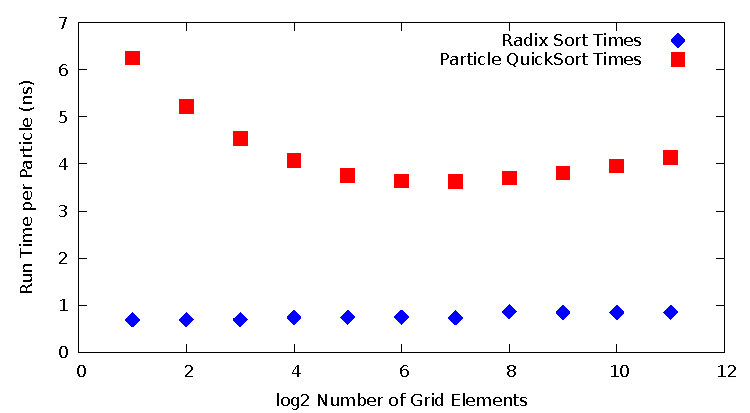
\includegraphics[width=5in]{design/sort_compare.pdf}
\end{center}
\caption{Comparison of Stantchev Sort and the thrust radix sort.}
\label{fig:stantchev_sort_compare}
\end{figure}

The data shown in figure \ref{fig:stantchev_sort_compare} was generated using a simple code that populates a partially ordered particle list and then sorts this list. The amount of data for each particle is similar to that of sceptic3D, six floats for position and velocity, and one integer to keep track of bin index. The ``grid" is represented by a series of bins, there is no need to represent individual cells for this comparison. The partially ordering is achieved by looping over the particle list and assigning each particle $p_i$ to bin $\mathrm{floor}(\frac{N_{part}}{G} i)$. Where $N_{part}$ is the total number of particles, $G$ is the size of the grid, and $i$ is the particle index. The ``partial" part of the ordering is achieved by drawing a random number for each particle, if this number is less than $R$, then a second random number is drawn to determine if the particle is being placed in the previous or next bin. The boundary conditions are periodic such that particles in bin 0 that are being placed in a lower bin end up in bin $G-1$ and particle in bin $G-1$ that are being shifted up will end up in bin 0. The number $R$ can be adjusted in order to adjust the fraction of particles that are moving. For the data shown in figure \ref{fig:stantchev_sort_compare} $R = 0.2$, $N_{part} = 2^{24}$, and G ranges from $2^1$ to $2^{12}$. 

Overall the thurst sort has the benefits of being easy to implement, very general, and is part of an externally maintained library that will be updated as GPU hardware changes. Fortunately the thrust sort is also much faster than the radix sort from the NVIDIA GPU Computing SDK 3.1. The performance of the thrust sort is fast enough that it is no longer the dominant cost. The downside to this sort is that it also requires allocation of buffer memory. The amount of memory required for this buffer array can be reduced by using separate arrays for each element of the particle list, which will be discussed in more detail in the next section. For now the thrust sorts benefits of simplicity and ``fast enough" make it the winner of the particle sort competition. 

\subsection{Spatial Indexing}

One way that the sort performance can be improved is through the use of space filling curves, such as a Z-order curve for cell-cluster indexing. Utilizing a space filling curve for the cluster indexing preserves the spatial ordering of the clusters in their layout in memory. This aids the sort by reducing the distance that particles must move in memory whenever they change clusters. We will use a z-order curve to index the cell clusters, since it is fairly simple to implement and will provide some performance boost to the code.

%%%%%%%%%%%%%%%%%%%%%%%%%%%%%%%%%%%%
	\section{Particle List Structure}
%%%%%%%%%%%%%%%%%%%%%%%%%%%%%%%%%%%%

Another major design question is what kind of data structure should be used for the particle list. In the serial version of sceptic3D the particle data is laid out in a 6xN array of reals in fortran. In C this layout corresponds to an array of six element structures. The array of structures formant performs well on the CPU since only one particle is being operated on at a time, this means that data from only a single particle will be required at a given time. On the GPU things are a bit different. When a data access is performed on the GPU a group of 32 threads, a warp, executes memory requests for the same element, but from 32 different particles. If these addresses are not sequential then the request will be divided up into as many 128 byte cache-line transactions as it takes to fulfill the requests from all 32 threads. In kernels where all six elements will be used soon after one another, such as in the move kernel, this is not a big issue. When the request for the first element is read from global memory, the data for the other 5 elements will also be retrieved from global memory. For the most part cache hits are almost as fast as registers, so subsequent requests for the other 5 elements will result in fast cache hits. Unfortunately this is not true of kernels in which only a subset of the elements is required, such as when calculating the particle bin index of each particle with relies only on the particles position. \cite{NVIDIACorporation2011}

\begin{figure}
\begin{lstlisting}[frame=single]
class XPchunk // Array of Structures
{
public:
	float x,y,z,vx,vy,vz;
};

class XParray // Structure of Arrays
{
public:
	float* x,y,z,vx,vy,vz;
};
\end{lstlisting}
\caption{Array of Structures and Structure of Arrays}
\end{figure}   
	
	The alternative is to use a structure of arrays, which corresponds to the transpose of the particle list structure in the fortran version of sceptic3D. The main benefit of a structure of arrays is that reading in a single element of the particle list for 32 particles corresponds to a 128 byte transfer, the size of the cache line transaction. None of the bandwidth is wasted. This only takes 6 reads to global memory, no reads to cache. Reading in the elements of the array of structures results in at least 6 reads to global memory for the first element, followed by 5 reads from cache in the best case scenario. In order to test this we ran our toy GPU PIC code with both an array of structures (AoS) and a structure of arrays (SoA). The results of this test are shown in table \ref{tab:struct_compare}. 
	
\begin{figure}[h]
\begin{center}
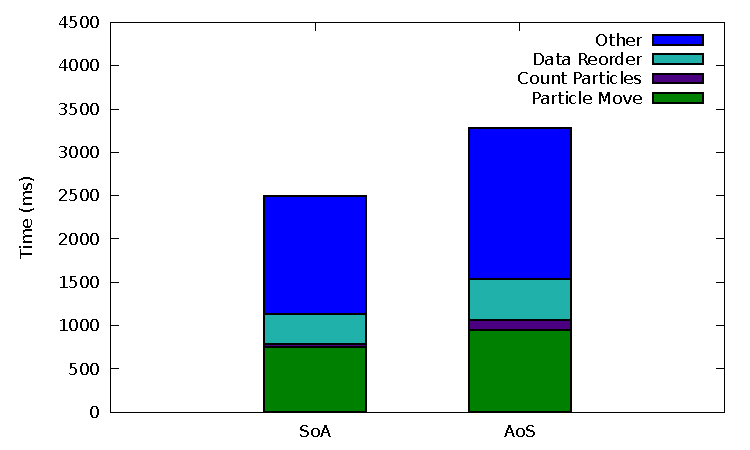
\includegraphics[width=5in]{design/soa_vs_aos.pdf}
\end{center}
\caption{Execution times of main steps for Array of Structures and Structure of Arrays. Count Particles and Data Reorder are steps used for a sorted particle list. Count Particles counts the number of particles in each sub-domain. Data Reorder reorders the particle list data after the binindex / particle ID pair have been sorted by the radix sort.}
\label{tab:struct_compare} 
\end{figure}



An additional benefit to using the the structure of arrays is the smaller buffer required for the particle sort. Using a structure of arrays we only need a 1xN array of floats to sort each element of the particle list into. We would need a 6xN floats for sorting the array of structures. This approach scales well with more complicated particles that must keep track of more information. For sceptic3D we have a total of 6 floats for spatial and velocity components, one 32-bit integer for the particle index, one float to keep of previous time step for reinjections, and a 16-bit integer for the binID. Using a structure of arrays the memory requirements imposed by the sorting step only increase the memory required per particle by 12\%. The standalone buffer array can also be useful for other uses, such as stream compactions and reductions of diagnostic outputs. 

The main downside of the structure of arrays approach is that a transpose is required for particle data transfers between the fortran sceptic3D code and the GPU code. Performing this transpose on the GPU would require a large amount of memory, which would reduce the total number of particles that could be run. Performing it on the CPU will be more costly computationally, but will provide better performance overall.  




%%%%%%%%%%%%%%%%%%%%%%%%%%%%%%%%%%%%
	\section{Particle Advancing}
%%%%%%%%%%%%%%%%%%%%%%%%%%%%%%%%%%%%
	Implementing sceptic3D's particle advance on the GPU is fairly straightforward, and for the most part is identical to the CPU implementation. The primary design challenge here is dealing with reinjections.

The sceptic3D particle advance algorithm is as follows:

\begin{algorithm}
	\begin{algorithmic}
		\FORALL{$p_i \in$ particles}
		\STATE $p_i \leftarrow \mathrm{move}(p_i,\Delta t)$
		\WHILE{$p_i\rightarrow \mathbf{x} \notin \mathrm{Domain}$}
			\STATE $\Delta t_{prev} \leftarrow \Delta t - \frac{\|\mathbf{\mathrm{exit}} - \mathbf{x}_i^0\|}{\|\mathbf{v}_i\|}$
			\STATE $p_i \leftarrow \mathrm{Reinject}()$
			\STATE $p_i \leftarrow \mathrm{move}(p_i,\Delta t_{prev})$
		\ENDWHILE	
		\ENDFOR
	\end{algorithmic}
	\caption{Sceptic3D Particle Advancing}
	\label{alg:padvnc}
\end{algorithm}

Reinjections on the CPU are performed whenever a particle leaves the computational domain. When this event occurs, the code first determines the exact point during the timestep that the particle left the grid. From there a new particle is reinjected by calculating a new position and velocity as described in \cite{Patacchini2007}. The new particle is then advanced the remainder of the times step, performing a second reinjection if the new particle also leaves the domain. 

Unfortunately this method does not work well on the GPU. If this same algorithm were to be used on the GPU it would result in a large amount of warp divergence. Calculating new random positions and velocities is also expensive. Ideally we would have all of the particles be moved, and then operate on the subset of particles that need to be reinjected. In CUDA this is done by compacting the particle stream down to a list that contains only particles that are undergoing reinjection. This compacted particle list is still a particle list, and can be advanced in the same manner as the main list.  





